\myChapter{Service Layer}\label{chap:servicelayer}
In diesem Kapitel sollen das Konzept  des Service Layer als gemeinsame
Schnittstelle einer Anwendung für alle übergeordneten Schichten besprochen
werden. Im zweiten Teil des Kapitels werden dann einige Implementierungen von
Service Funktionalitäten vorgestellt, die in verschiedenen Anwendungsfällen
einsetzbar und wiederverwendbar sind.

\section{Definition}
Der Presentation Layer einer Anwendung bietet die Möglichkeit, die
Anwendungslogik auf verschiedenen Wegen verfügbar zu machen. So zum Beispiel
über eine grafische Anwenderoberfläche, eine Webanwendung, eine
Kommandozeilenanwendung oder einen Dateneinspieler sowie über verschiedene
\ac{RPC} Protokolle\footnote{Der dafür hergeleitete Remoting Layer wird in
Kapitel \ref{chap:remotinglayer} näher behandelt}. Um eine Duplizierung von
Anwendungslogik zu vermeiden ist es sinnvoll, für diese Möglichkeiten eine
einzige gemeinsame Schnittstelle der Anwendung zu definieren, die auch als
\emph{Service Layer} (vgl. \cite{fowler:2002} S. 133) bezeichnet wird. Für den
Benutzer des Service Layer werden somit alle verfügbaren Operationen der Anwendung an
einer zentralen Stelle und mit einer möglichst einfachen Schnittstelle definiert.

Einzuordnen ist der Service Layer in der Schicht der Anwendungslogik
über dem Domain Layer, wie Abbildung \ref{ill:servicelayer} zeigt.

\begin{figure}[bth]
    \center{\includegraphics[width=\linewidth]{images/overviews/service}}
	\caption{Einordnung des Service Layer}
	\label{ill:servicelayer}
\end{figure}

\subsection{Implementierungmöglichkeiten}
Analog zu dem in Abschnitt \ref{sec:domainmodel} beschriebenen Möglichkeiten für
die Implementierung von Anwendungslogik im Domain Model gibt es auch für den
Service Layer zwei verschiedene Implementierungsansätze (vgl.
\cite{fowler:2002} S. 134).

Bei der \emph{Domain Model Facade} implementieren die Service Layer Klassen
selbst keine Anwendungslogik, sondern dienen lediglich als Vermittler zwischen
dem Domain Model und dem Benutzer des Service Layer. Dadurch muss sich der
Benutzer nicht mit der Verwendung des möglicherweise sehr komplexen Domain Model
befassen, sondern kann die meist deutlich einfacher strukturierte
Schnittstelle des Service Layer verwenden.

Durch die Einführung des Service Layer als Schicht über dem Domain Model bietet
sich aber auch die Möglichkeit an, die Anwendungslogik ebenfalls entsprechend zu
organisieren. Hierbei unterscheidet der \emph{Opera\-tion Script} Ansatz
zwischen der allgemeinen Anwendungslogik, die in den Service Klassen implementiert wird,
und Anwendungslogik, die weiterhin in Domain Klassen gehalten werden sollte und
deshalb an diese weitergeleitet wird. Die Implementierungen einzelner Service
Klassen fassen dabei zusamengehörige Bereiche der Anwendungslogik zusammen.

\subsection{Umsetzung}
Die für den Service Layer benötigten Methoden sind relativ einfach herzuleiten,
da sie sich direkt nach den Anforderungen der direkt übergeordneten Schichten
richten. Die wichtigste übergeordnete Schicht ist hier normalerweise eine
\emph{Anwenderoberfläche}, weshalb sich die Service Layer Methoden in erster
Linie nach den Operationen ausrichten, die dort benötigt werden. Auch wenn die
dafür notwendige Anwendungslogik sehr komplex sein kann, lassen sie sich aus
Sicht der Schnittstelle in den meisten Fällen auf einfache \ac{CRUD}
Funktionalitäten reduzieren. Trotz der Ausrichtung der Service Methoden nach der
übergeordneten Schicht sollte die Implementierung des Service Layer weiterhin
unabhängig davon erfolgen. Das heißt, dass der Service Layer selbst keine
Kenntnis diese Schichten benötigen sollte.

Schwieriger gestaltet sich die Abstraktion in passende Service Layer Klassen. Für
kleinere Anwendungen kann es ausreichend sein, eine einzige Service Layer Klasse
zu implementieren, die nach der Anwendung selbst benannt ist und alle notwendigen
Operationen bereitstellt. Bei größeren Anwendungen gibt es die Möglichkeit, für
verschiedene Teilbereiche der Anwendung jeweils eine Service Klasse zu
implementieren. Ebenso ist es möglich, verschiedene Teilbereiche des Domain
Model in je einer Service Klasse zu implementieren.

Auch wenn die tatsächliche Implementierung der Anwendungslogik in einer Service
Klasse erfolgt, sollte die Definition der Service Layer Schnittstelle in Form von
\emph{Service Interfaces} erfolgen. Dafür wird ein Java Interface erstellt, das
dann von einer Service Klasse implementiert wird. In Verbindung mit Dependency
Injection muss der Benutzer dadurch lediglich Kenntniss über das Service
Interface haben und kann dieses verwenden, während die implementierende Klasse
problemlos ausgetauscht werden kann. Ist die Implementierung einer Service Klasse
von einem anderen Service abhängig, sollte auch dort das entsprechende Interface
verwendet werden.

\begin{figure}[bth]
    \center{\includegraphics[width=\linewidth]{images/serviceexample}}
	\caption{Beispiel eines Service Layer Interfaces und einem \ac{DAO}}
\end{figure}

\section{Implementierungen}
Durch die in Abschnitt \ref{chap:introduction} vorgestellten Eigenschaften einer
Anwendung stellen sich auch verschiedene Anforderungen an die Implementierung des
Service Layer. Viele der benötigten Funktionalitäten werden in verschiedenen
Anwendungen in einer ähnlichen Form benötigt und eignen sich deshalb sehr gut für
eine generische Implementierung in Form einer Klassenbibliothek. Deshalb sollen
in den folgenden Abschnitten Service Interfaces und entsprechende Implementierungen
vorgestellt werden, die einige dieser Aufgaben übernehmen.

\subsection{Anwendungscaches}\label{service:cache}
Anwendungscaches sind Zwischenspeicher, die Daten, die der Anwendung bereits
vorlagen, speichern, um sie bei einem neuerlichen Zugriff schneller zur Verfügung
stellen zu können. Das ist vor allem in Anwendungen sinnvoll, die eine hohe Zahl
an Anfragen verarbeiten müssen und sich die bereitgetellten Daten im Verhältnis
dazu selten ändern. Entsprechend der Definition von Unternehmensanwendungen ist
das sehr häufig der Fall. Kommuniziert die Anwendung mit anderen entfernten
Systemen, kommt hinzu, dass die direkte Abfrage von Daten meist mit mehr Aufwand
verbunden ist, als es bei dem Zugriff auf einen Cache der Fall ist. Dazu zählt
grundsätzlich jede Abfrage, die eine Netzwerkkommunikation benötigt, da schon die
Übertragung der Daten eine gewisse Zeit in Anspruch nimmt. Ist die entfernte
Anwendung eine Datenbank, sollte ebenfalls jede überflüssige Abfrage vermieden
werden, um die Ressourcen des Datenbankservers für die tatsächlich anfallende
Arbeitslast zur Verfügung zu haben. Das gilt auch, wenn durch die entfernte
Anwendung andere umfangreiche Berechnungen vorgenommen werden und die
Wahrscheinlichkeit hoch ist, dass das Ergebnis mehrmals abgefragt wird. Da die
Kommunikation mit anderen entfernten Anwendungen auch mit zusätzlichen Kosten
verbunden sein kann, lassen sich durch einen sinnvoll eingesetzten Cache auch
Kosten sparen.

\subsubsection{Verdrängungsstrategien}
Auf der anderen Seite wird von einem Cache wiederum ein schneller Datenspeicher
benötigt, der ebenfalls mit zusätzlichen Kosten verbunden ist. Hier muss ein
passender Kompromiss zwischen Kosten und Größe des Cache Speichers gefunden
werden. Dies führt in den meisten Fällen dazu, dass der verwendete Cache deutlich
kleiner ausfällt als die Gesamtheit der Daten die eine Anwendung zur Verfügung
stellen kann. Werden neue Daten in den Cache gelegt, wenn dieser bereits voll
ist, können verschiedene Verdrängungsstrategien zur
Anwendung kommen (vgl. \cite{wiki:cachealgorithms}):

\begin{description}
	\item[Optimal] Auch \emph{Belady's Verfahren} genannt, ist eine optimale 
	Verdrängungsstrategie, die immer das Element aus dem Cache entfernt, auf das
	in der Zukunft am seltensten zugegriffen wird. Das ist aber nur möglich, wenn
	der gesamte Ablauf eines Programms im Voraus bekannt ist. Da dies
	normalerweise in keiner Anwendung der Fall ist, kann diese
	Verdrängungsstrategie nicht direkt implementiert werden. Ein optimaler Cache
	eignet sich aber gut als Vergleich für andere Verdrängungsstrategien.
	\item[First In First Out (FIFO)] Das erste Element das in den Cache eingefügt
	worden ist wird auch als erstes verdrängt. Die dafür notwendige Datenstruktur
	ist sehr einfach aufgebaut und kann sehr performant implementiert werden. Eine
	FIFO Verdrängungsstrategie liefert aber nur in seltenen Fällen gute
	Ergebnisse.
	\item[Least Recently Used (LRU)] Das Element, auf das am längsten nicht
	zugegriffen wurde, wird aus dem Cache verdrängt. Hierbei muss eine
	Datenstruktur benutzt werden, die den Zeitpunkt des letzten Zugriffs auf ein
	Cache Element speichert und danach sortiert. Das
	erste Element in dieser Liste wird dann als erstes verdängt.
	\item[Least Frequently Used (LFU)] Das am seltensten gelesene Element wird aus
	dem Cache verdrängt. Entsprechend einem LRU Cache wird eine Datenstruktur
	benutzt, die nach der Anzahl der Zugriffe sortiert ist. Auch hier wird dann das
	erste Element der Liste zuerst verdrängt.
\end{description}

Die Optimierung der Cache Verdrängungsstrategie ist sehr anwendungsspezifisch
und erfordert umfangreiche Tests und Benchmarks. Da der Programmablauf in einem
Benchmark im Voraus bekannt ist, kann man hier einen optimalen Cache als
Vergleich zu der aktuellen Verdrängungsstrategie heranführen. Die Kriterien für die
Bewertung der Verdrängungsstrategie sind \emph{Cache Hits}, \emph{Cache Misses}
und \emph{False Positives}. Ein Cache Hit tritt auf, wenn das gesuchte Element im
Cache gefunden wurde, ein Cache Miss, wenn nicht. Bei einem Cache Miss muss das
gewünschte Ergebnis dann von der Anwendung selbst geliefert und in den Cache
gelegt werden. False Positives treten bei einem Cache Hit auf, wenn das
gespeicherte Element nicht mit dem eigentlichen Ergebnis der Anwendung konsistent
ist. Das ist der Fall, wenn sich der Zustand der Anwendung geändert hat, aber die
betroffenen Elemente im Cache nicht entfernt wurden. Hier kommt es auch auf die
Anwendung selbst an, ob False Positives für einen bestimmten Zeitraum akzeptabel
sind oder nicht.

\subsubsection{Cache Arten}
In netzwerkbasierten Anwendungen wird zwischen \emph{lokalen} und
\emph{verteilten} Caches unterschieden. Um eine möglichst einfache Schnittstelle
zur Verfügung zu stellen, werden Anwendungscaches als eine Art assoziatives
Array behandelt, wobei der Schlüssel ein eindeutiger Bezeichner\footnote{Hier
wird meist ein Hash Wert oder ein anderer eindeutiger String verwendet} des zu cachenden Elements und
der Wert das zu speichernde Element selbst ist. Bei einem lokalen Cache werden
die Cache Elemente im Arbeitsspeicher oder auf der Festplatte des Systems
gespeichert, auf dem auch die Anwendung selbst ausgeführt wird. Meist
existiert eine für die Programmiersprache native Schnittstelle, wodurch die
Einbindung in eine Anwendung entsprechend einfach ist. Ein verteilter Cache wird
über ein für diese Aufgabe passendes Netzwerkprotokoll angesprochen und kann
wiederum mit anderen entfernten Caches kommunizieren.

\subsubsection{Implementierung}
Durch die Key-Value Store Schnittstelle der Cache Implementierungen muss das
Cache Service Interface lediglich die dafür üblichen Operationen \emph{get(key)},
\emph{put(key, value)} und \emph{remove(key)}
bereitstellen. Um die Generierung eindeutiger Schlüssel zu vereinfachen, wurde
außerdem ein \emph{Region} Parameter eingeführt, das den Cache in virtuelle
Namensräume aufteilt oder - je nach Implementierung - dazu dient, verschiedene
Caches anzusprechen. Wird das Cache Service Interfaces konsequent im gesamten
Service Layer verwendet, ist ein problemloser Wechsel zu einem anderen Cache
System möglich.

Bei der Verwendung eines Cache müssen die betroffenen Stellen den Service
Implementierungen angepasst werden. Da die Anwendung ausschließlich über die
Schnittstelle des Service Layer verwendet wird, wäre es grundsätzlich möglich,
alle Ergebnisse der Methodenaufrufe in einem Cache zwischenzuspeichern. Aus einem
Service Layer Methodenaufruf ließe sich problemlos ein eindeutiger Schlüssel
generieren, unter dem das Ergebnis im Cache abgelegt wird. Anhand der
Methodenaufrufe ist aber meist nicht erkennbar, ob und wie der Zustand der
Anwendung geändert wurde. Deshalb ist es kaum möglich festzustellen, welche
Elemente im Cache gelöscht werden müssten um False Positives zu vermeiden. Aus
diesem Grund bleibt die Verwendung des Cache Service weiterhin dem Entwickler
überlassen. In dem Pseudocode Beispiel in Listing \ref{lst:cacheuse} wird die
Verwendung des Cache Service Interface illustriert.
\pagebreak
\lstset{language=Pascal}
\lstinputlisting[caption=Pseudocode für die Verwendung des Cache
 Service, label=lst:cacheuse] {sources/usecache.pseudo}

Das Cache Service Interface wurde für das lokale Cache System EhCache
und den verteilten Cache Memcached implementiert.

\begin{description}
\item[EhCache] EhCache\footnote{\url{http://ehcache.org/}} ist grundsätzlich ein
lokaler Cache für Java, der im Arbeitsspeicher der Anwendung arbeitet, aber auch
Daten auf der Festplatte ablegen kann. Durch die Möglichkeit, die Cache Inhalte
über ein Netzwerk zu replizieren, ist auch die Verwendung als verteilter Cache
möglich. Für die Verwendung als verteiltert Cache bietet der EhCache Hersteller
Terracotta\footnote{\url{http://www.terracotta.org/}} auch kommerzielle Lösungen
an.
\item[Memcached] Memcached\footnote{\url{http://memcached.org/}} ist ein
verteilter Cache, der die Daten normalerweise im Arbeitsspeicher der Cache Server
ablegt. Memcached ist einfach zu verwenden und hat sehr gute
Skalierungseigenschaften, weshalb es vor allem bei großen Webapplikationen
eingesetzt wird um die Datenbanken zu entlasten. So betrieb das soziale Netzwerk
Facebook\footnote{\url{http://facebook.com}} Ende 2008 ein aus 800 Servern
bestehendes Memcached Cluster, das insgesamt 28 TB RAM als Cache zur Verfügung
stellte (siehe \cite{saab:2008}).
\end{description}

\begin{figure}[bth]
    \center{\includegraphics[width=0.8\linewidth]{images/cacheservice_uml}}
	\caption{UML Diagramm des Cache Service und Implementierungen}
\end{figure}

\subsection{Domain Model Zugriff}\label{service:domainmodel}
Eine der wichtigsten Aufgaben des Service Layer ist es, dem Benutzer Zugriff auf
die im Domain Model verarbeiteten Daten zu ermöglichen. Auch wenn die
Verarbeitung dieser Daten in der Anwendung selbst mit komplexer Anwendungslogik
verbunden sein kann, handelt es sich bei den nach außen hin benötigten Methoden
um grundlegende \ac{CRUD} Funktionalitäten. Die Hauptaufgabe eines Service zur
Domain Model Verwaltung ist also das \emph{Erstellen}, \emph{Lesen},
\emph{Aktualisieren} und \emph{Löschen} von Domain Objekten.

In den meisten Fällen kommt zur dauerhaften Speicherung des Domain Models ein
\ac{RDBMS} zum Einsatz, häufig in Verbindung mit einem \ac{ORM} Framework. In
diesem Fall sind die Domain Objekte auch gleichzeitig Entitäten, die in einem
\ac{RDBMS} abgelegt werden. Die \ac{CRUD} Funktionen auf einem Domain Objekt
werden dann normalerweise in den entsprechenden Aufruf auf der Datenbank
umgesetzt.

\begin{description}
	\item[Erstellen und Aktualisieren] Beide Operationen sind sich meist sehr
	ähnlich. Die Entscheidung, ob ein übertragenes Domain Objekt angelegt oder
	aktualisiert werden muss, wird normalerweise anhand des eindeutigen
	Bezeichners getroffen, sofern dieser vorhanden ist. Ist er nicht
	gesetzt, muss das Domain Objekt neu angelegt werden, ansonsten wird das
	Domain Objekt mit dem entsprechenden Bezeichner aktualisiert. Bei
	beiden Operationen sollte immer eine Validierung aller betroffenen Domain
	Objekte vorgenommen werden.
	\item[Lesen] Im einfachsten Fall wird ein Domain Objekt anhand seines
	eindeutigen Bezeichners gelesen. Auch die Auflistung von Domain
	Objekten anhand verschiedener Auswahlkriterien muss ermöglicht werden.
	\item[L\"oschen] Entfernt ein Domain Objekt mit einem eindeutigen Bezeichner.
\end{description}

\subsubsection{Grails ORM}
\ac{GORM} ist eine Erweiterung des \ac{ORM} Frameworks Hibernate für die
Programmiersprache Groovy. Es ist Teil des Webframeworks
\emph{Grails}\footnote{\url{http://grails.org}}, kann aber inzwischen auch
unabhängig davon benutzt werden. Deshalb soll hier auf die Details von Grails
selbst nicht weiter eingegangen werden. Durch die dynamischen Eigenschaften von
Groovy entstehen einige neue Möglichkeiten den Zugriff auf Domain Objekte, die
von Hibernate verwaltet und in einem \ac{RDBMS} abgelegt werden, zu vereinfachen.
So erstellt \ac{GORM} automatisch verschiedene \ac{CRUD} Methoden, die direkt auf
den Domain Objekten verwendet werden können und übernimmt somit auch Aufgaben der
\ac{DAO} Klassen. Methoden, die zum Lesen des Domain Objekts verwendet werden,
sind hierbei statische Methoden auf der Domain Klasse. Methoden zum Speichern und
Löschen werden auf dem betroffenen Domain Objekt selbst aufgerufen. Listing
\ref{lst:gorm} zeigt ein Beispiel für die Verwendung von \ac{GORM}.

\lstset{language=Java}
\lstinputlisting[caption=Beispiel für die Verwendung des GORM, label=lst:gorm]
{sources/domainexample.groovy}
 
\subsubsection{Implementierung}
In der Implementierung des Domain Model Services konnten durch die gute
gegenseitige Integration von Groovy und Java die Vorteile einer dynamischen
Sprache mit denen der statischen Typisierung optimal miteinander verbunden
werden. Ein Service Interface muss als eindeutige, statische Schnittstelle
definiert werden, weshalb es nicht möglich ist, die dynamisch durch \ac{GORM}
erstellten Methoden direkt anzubieten. Die Beschreibung einer Service
Schnittstelle erfolgt deshalb weiterhin als Java Interface. Da Groovy aber ein
Java Interface zur Laufzeit implementieren kann, ist es möglich, Aufrufe auf
dieses Interface an die von \ac{GORM} erstellten Methoden weiterzuleiten. Somit
wird die Anforderung des Service Layer an ein eindeutiges Interface erfüllt, es
ist aber gleichzeitig möglich, die dynamisch erstellten Methoden zu verwenden.
Diese Möglichkeit bleibt auch bestehen, wenn Groovy nicht direkt zur
Implementierung des Service Layer verwendet wird\footnote{Die Groovy
Klassenbibliotheken müssen aber zur Verfügung stehen}. Der Entwickler muss
lediglich das gewünschte Service Interface definieren, das den \ac{GORM}
Konventionen für die Benennung der dynamischen Methoden folgt, wie in Listing
\ref{lst:domainserviceexample} gezeigt.

\lstset{language=Java}
\lstinputlisting[caption=Beispiel eines Domain Model Service Interface,
label=lst:domainserviceexample] {sources/domainserviceexample.java}

Listing \ref{lst:springdomainexample} zeigt ein Beispiel, für die Spring
Context Definition zur Verwendung des Service. Eine Klasse, die das Service
Interface implementiert ist nicht notwendig.

\lstset{language=XML}
\lstinputlisting[caption=Verwendung des Domain Model Service in einem Spring
Context, label=lst:springdomainexample] {sources/domainexample.xml}

Werden Listen von Domain Objekten ausgelesen, möchte man die zurückgelieferten
Elemente oft nach verschiedenen Kriterien sortieren und die Größe der
zurückgelieferten Liste beschränken und navigierbar machen. Dieser Vorgang wird
auch \emph{Paging} genannt. Die Implementierung des Paging stellt einen gewissen
Zusatzaufwand dar, da jede Methode, die eine Liste von Domain Objekten
zurückliefert entsprechend angepasst werden muss. Um die Arbeit damit etwas zu
erleichtern, wurde eine \emph{Pager} Klasse implementiert, die Informationen
darüber enthält, welcher Bereich der Auflistung angefordert wird und nach welchen
Kriterien die Elemente sortiert werden sollen. Für Service Methoden die an eine
\ac{GORM} Methode weiterleiten und mit einem Pager als Parameter definiert
werden, wird das Paging automatisch vorgenommen. Soll Paging auch in anderen Methoden
angewendet werden, muss das Pager Objekt dort programmatisch eingebunden werden.
Dies kann man entweder direkt auf Ebene der Datenbankabfrage oder im Nachhinein auf
der zurückgelieferten Liste der Domain Objekte umsetzen.

\begin{figure}[bth]
    \center{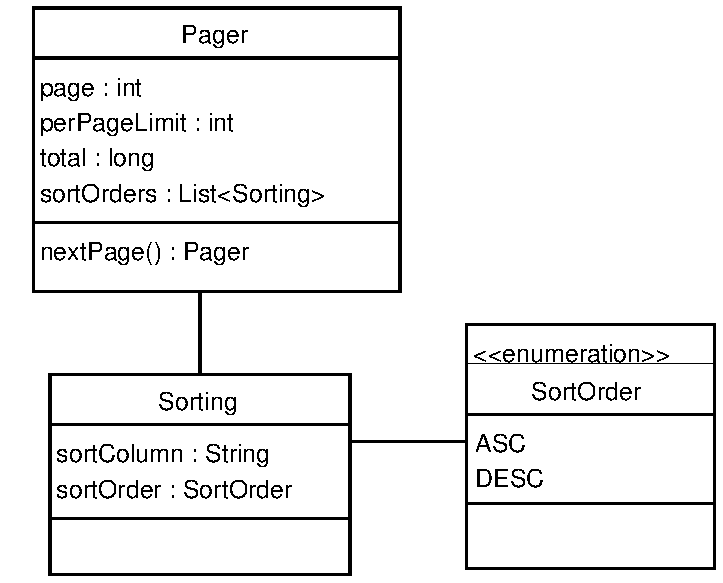
\includegraphics[width=0.7\linewidth]{images/pager_uml}}
	\caption{UML Diagramm der Paging Klassen}
\end{figure}

\subsection{Benutzerverwaltung}\label{service:security}
Da eine Anwendung fast ausnahmslos von mehreren Benutzern verwendet wird, müssen
sie in irgendeiner Form eindeutig identifizierbar sein. Auch hier stellt der Service
Layer wieder einen guten Ansatzpunkt dar, um die Aufgaben der Authentifizierung
und Autorisierung zu übernehmen.

\begin{description}
\item[Authentifizierung] Authentifizierung ist der Vorgang, einen Benutzer
eindeutig zu identifizieren und sicherzustellen, dass es sich um den
behaupteten Teilnehmer handelt. Grundsätzlich wird zwischen drei verschiedenen
Arten der Authentifizierung (vgl. \cite{kruth:2004} S. 295) unterschieden.
\begin{itemize}
\item Bei der Authentifizierung durch \emph{Wissen} handelt es sich
üblicherweise um die Kombination aus Benutzername und Passwort.
\item Ein Teilnehmer authentifiziert sich durch \emph{Besitz}, wenn er ein
Objekt mit den entsprechenden Authentizitätsinformationen besitzt,
beispielsweise eine Chipkarte.
\item Ferner ist es möglich, dass sich ein Teilnehmer durch
\emph{unveränderliche Eigenschaften}, wie zum Beispiel die biometrische
Eigenschaft eines Fingerabdrucks, authentifizieren kann.
\item Auch eine Kombination der verschiedenen Authentifizierungsmechanismen ist
möglich.
\end{itemize}
\item[Autorisierung] Berechtigungen werden von einem Administrator der Anwendung
vergeben und bestimmen, ob ein authentifizierter Teilnehmer auf bestimmte Domain
Objekte und Service Methoden zugreifen darf (vgl. \cite{kruth:2004} S. 292). Der
Vorgang der Überprüfung, ob ein Teilnehmer die benötigten Berechtigungen hat,
wird \emph{Autorisierung} genannt. Berechtigungen auf Domain Objekten hängen in den
meisten Fällen direkt mit den darauf auszuführenden \ac{CRUD} Operationen
zusammen. So dürfen manche Benutzer Domain Objekte lesen, erstellen und
verändern, während andere lediglich lesenden Zugriff darauf haben.
\end{description}

Die sichere Beschaffung und Übertragung der für die Authentifizierung eines
Benutzers notwendigen Informationen zum Service Layer ist weiterhin Aufgabe des
Benutzers.

\subsubsection{Spring Security}
Spring Security (vormals Acegi Security) ist ein Unterprojekt des Spring
Frameworks, das umfangreiche Möglichkeiten für die Authentifizierung
und Autorisierung von Benutzern bietet. Einige nennenswerte
Protokolle zur Benutzerauthentifizierung sind:

\begin{description}
	\item[LDAP] LDAP ist eine vor allem in großen Unternehmen häufig genutzte
	Möglichkeit, auf zentral gespeicherte Benutzerinformationen zugreifen zu
	können.
	\item[HTTP Authentifizierung] Auch die im \ac{HTTP} Protokoll
	spezifizierten Authentifizierungsmechanismen werden unterstützt.
	\item[OpenID] OpenID ist ein dezentralisierter, offener Standard für die
	Benutzerauthentifizierung. An einem Authentifizierungsvorgang beteiligt sind
	die Anwendung selbst, der zu authentifzierende Benutzer und ein OpenID
	Anbieter, bei dem der Benutzer seine Zugangsinformationen gespeichert hat.
	\item[UserService] Spring Security bietet auch die Möglichkeit, ein
	eigenes UserService Interface zu implementieren. Dadurch kann die Anwendung
	die für die Authentifizierung notwendigen Informationen selbst bereitstellen.
\end{description}

Hat sich ein Benutzer erfolgreich authentifiziert, legt Spring Security diese
Informationen in einem \emph{SecurityContext} ab, der dann in der gesamten
Anwendung verfügbar ist.

Ist der Context erstellt, also der Benutzer authentifiziert, bietet Spring
Security verschiedene Möglichkeiten zur Autorisierung der vom Benutzer
duchgeführten Aktionen. Unterstützt wird eine \emph{rollenbasierte
Authorisierung} (vgl. \cite{park:2001}), auf dessen Grundlage Service
Methoden oder einzelne Domain Objekte geschützt werden können. Die Grundidee der
rollenbasierten Authorisierung ist, dass Berechtigungen mit
Rollen\footnote{Mögliche Rollen sind beispielsweise Administrator, Manager, User
usw.} verbunden sind und den Benutzern dann diese Rollen zugewiesen werden.

\subsubsection{Implementierung}
Der Service zur Benutzerverwaltung übernimmt zwei Aufgaben. Zum Einen
die Administration von Benutzern und Rollen, zum Anderen die
Authentifizierung und Authorisierung eines Benutzers. Neben der Erstellung und
Implementierung des entsprechenden Service Interface ist es deshalb auch
notwendig, von \ac{GORM} verwaltete Domain Klassen für Benutzer und Rollen zu
erstellen. Abbildung \ref{ill:securitymodel} zeigt das entsprechende Domain
Model und die Interfaces, die aus dem Spring Security Framework verwendet
wurden.

\begin{figure}[bth]
    \center{\includegraphics[width=\linewidth]{images/securitymodel}}
	\caption{Benutzer und Rollen Domain Model mit Spring Security}
	\label{ill:securitymodel}
\end{figure}

Da der Service Layer unabhängig von seinen Benutzern als eigene Schicht arbeiten
soll, übernimmt er keine implementierungsspezifischen Aufgaben des verwendeten
Authentifizierungsmechanismus. Ist der Benutzer beispielsweise eine
Weboberfläche, muss die Umwandlung von der dort verwendeten \ac{HTTP} Authentifzierung in einen
Security Service Methodenaufruf bereits dort erfolgen. Abbildung
\ref{ill:securityservice} zeigt die Methoden des Security Service Interface.

\begin{figure}[bth]
    \center{\includegraphics[width=0.6\linewidth]{images/securityservice}}
	\caption{Security Service Interface}
	\label{ill:securityservice}
\end{figure}

\subsection{Logging und Monitoring}\label{service:logging}
Dadurch, dass eine Unternehmensanwendung von vielen Benutzern verwendet wird und
im Normalfall auch mit anderen entfernten Anwendungen kommuniziert, können
Fehler auftreten, die nicht immer direkt nachvollziehbar sind. Deshalb ist es
sinnvoll, den Programmablauf zu protokollieren, um Fehler leichter zu
lokalisieren und auch das Nutzungs- und Laufzeitverhalten besser nachvollziehen zu können. Dies wird
allgemein \emph{Logging} genannt. In lokalen Anwendungen können Debugger, die
eine Übersicht über den Zustand der Anwendung ermöglichen, für die Fehlersuche
verwendet werden. In verteilten Systemen, die über entfernte Methodenaufrufe
kommunizieren, ist diese Möglichkeit der Fehlersuche nicht mehr in dieser Form
realisierbar. Hier können aber Statusmeldungen durch Logging hilfreich sein, um
den Fehler auch in solchen Anwendungen besser eingrenzen zu können und die
Administratoren über aufgetretene Fehler zu informieren. Das Logging der
Ausführungszeiten einzelner Methoden kann außerdem dabei helfen die Laufzeit der
Anwendung zu optimieren. Auch die Auswertung des Benutzerverhaltens ist eine
wichtige Aufgabe des Loggings. Dadurch lassen sich Rückschlüsse führen
wie die Anwendung tatsächlich verwendet wird und verbessert werden kann.

Hinzu kommt der Trend, dass die Bezahlung für die Benutzung einer Anwendung
individuell nach dem tatsächlichen Nutzungsvolumen erfolgt (vgl.
\cite{brandon:2009}). Um dies zu ermöglichen bietet sich der zentrale Logging
Mechanismus ebenfalls an. Durch die Auswertung der protokollierten
Benutzeraktivitäten lässt sich dann eine nutzungsbezogene Rechnung stellen.

\subsubsection{Logging Frameworks für Java}
Es gibt eine Vielzahl an Logging Frameworks für Java, die aber meist ähnlichen
Ansätzen folgen. So werden mehrere Log Level\footnote{Üblich sind FATAL, ERROR,
WARN, INFO und DEBUG} unterstützt, für die Nachrichten bzw. Exception Objekte
protokolliert werden können. Auch ist es möglich, Logger an verschiedene
Ausgabesysteme anzubinden. Normalerweise handelt es sich dabei um eine Datei,
aber auch die Anbindung an eine Datenbank oder die Versendung von Nachrichten bei einem
bestimmten Log-Ereignis sind möglich. Idealerweise soll ein Framework nicht
direkt von der tatsächlichen Implementierung eines der vielen Java Logging
Frameworks abhängig sein, sondern diese Entscheidung dem Benutzer überlassen. Zu
diesem Zweck wurde das \ac{SLF4J}\footnote{\url{http://www.slf4j.org}}
entwickelt, das entsprechend dem \emph{Facade Design Pattern} ein Logging Interface bereitstellt und Methodenaufrufe an die
vom Benutzer gewählte Logging Implementierung weiterleitet.

\subsubsection{Implementierung}
Die Implementierung des Logging Service stellt grundsätzlich die Methoden dieses
Interfaces zur Verfügung. Zusätzlich wurde der Logging Mechanismus um sogenannte
\emph{Actions} erweitert. Diese repräsentieren jeweils Ereignisse, die ausgeführt
werden, sobald sie durch den Logging Service protokolliert werden. Dadurch kann
die unmittelbare Rechnungsstellung von Benutzeraktionen ebenso realisiert werden
wie die Ausführung von bestimmten Wiederherstellungsoperationen bei einem
kritischen Fehler. Zu Optimierung der Laufzeit können Log Meldungen und Actions
außerdem durch den verwendeten Cache Service gepuffert werden, um zu einem
späteren Zeitpunkt ausgeführt oder geschrieben zu werden.

\subsection{Internationalisierung}\label{service:i18n}
Hat die Anwendung eine sehr große Zahl an Anwendern, kann es vorkommen, dass eine
Anpassung an unterschiedliche Kulturzonen und Sprachen der Anwender benötigt
wird. Das ist vor allem bei öffentlich zugänglichen Webanwendungen der Fall, die
auf einen internationalen Markt abzielen. Die Erfahrung hat gezeigt, dass der
Aufwand für die Internationalisierung oft unterschätzt wird. Der Service Layer
als gemeinsame Anwendungsschnittstelle kann hierbei ein guter Ansatz sein, um
die Anwendung internationalisierbar zu machen und den damit verbundenen
Mehraufwand minimal zu halten.

\subsubsection{Internationalisierung in Java und Spring}
Bei der Übersetzung in andere Sprachen ist es üblich, Strings, die in
verschiedenen Sprachen vorkommen können, durch einen eindeutigen Schlüssel zu
ersetzen. Ist die gewünschte Sprache bekannt, wird dieser Schlüssel dann durch
den entsprechenden Sprachtext ersetzt. Für die Internationalisierung bieten die
Java Standardbibliothek und das Spring Framework verschiedene Klassen an, die die
Arbeit damit erleichtern:

\begin{description}
\item[Locale]
Locale\footnote{\url{http://java.sun.com/javase/6/docs/api/java/util/Locale.html}}
Objekte stellen eine geografische, politische oder kulturelle Region dar. Sie
werden entsprechend den ISO Abkürzungen für
Sprachen\footnote{\url{http://www.loc.gov/standards/iso639-2/englangn.html}} und
Länder\footnote{\url{http://www.iso.ch/iso/en/prods-services/iso3166ma/02iso-3166-code-lists/list-en1.html}}
repräsentiert. Operationen, die aufgrund des übergebenen Locale Objekts regions-
und sprachspezifische Ergebnisse zurückliefern, werden auch locale-sensitiv
genannt. Locale Objekte werden meist nicht instanziiert, sondern von der
\ac{JVM} bereitgestellt, die eine Liste der installierten Sprachen und den entsprechenden
Locale Objekten mitführt.
\item[Format]
Format\footnote{\url{http://java.sun.com/javase/6/docs/api/java/text/Format.html}}
ist eine abstrakte Basisklasse um locale-sensitive Informationen zu formatieren.
Für die gängigen Anwendungsfälle stellt die Java Standardbibliothek die
folgenden Implementierungen bereit:
\begin{itemize}
  \item \emph{DateFormat} für die Formatierung von Datumsangaben
  \item \emph{NumberFormat} für die Formatierung von Zahlen unter
  Berücksichtigung der für die Locale üblichen Trennzeichen
  \item \emph{MessageFormat} um Nachrichten sprachunabhängig zusammenzusetzen
  und dann entsprechend einer \emph{Locale} zu formatieren
\end{itemize}
\item[ResourceBundle] Ein
ResourceBundle\footnote{\url{http://java.sun.com/javase/6/docs/api/java/util/ResourceBundle.html}}
ist eine abstrakte Basisklasse, die lokalisierte Objekte bereitstellt. Auf die
Objekte kann über die Kombination aus einem eindeutigen String (Schlüssel) und
dem Locale Objekt für die gewünschte Sprache zugegriffen werden.
\item[MessageSource] Eine
MessageSource\footnote{\url{http://static.springsource.org/spring/docs/3.0.x/javadoc-api/org/springframework/context/MessageSource.html}}
ist ein vom Spring Framework zur Verfügung gestelltes Interface, das den Zugriff
auf internationalisierte Nachrichten vereinfacht. Die bereitgestellten
Implementierungen verwenden das oben beschriebene \emph{ResourceBundle} um die
Nachrichten aufzulösen und das entsprechende \emph{MessageFormat} um diese zu
parameterisieren.
\end{description}

In der Standardimplementierung benutzt ein \emph{ResourceBundle} die von Java
unterstützten \emph{Property} Dateien. Für jeweils eine unterstützte Locale wird
eine Datei angelegt, die als Konvention das Kürzel der entsprechenden Locale am
Ende des Dateinamens enthält. In dieser Datei erfolgt dann die Zuordnung von
einem Schlüssel zu der passenden Übersetzung mit Platzhaltern für Inhalte, die
dynamisch eingefügt werden. Listing \ref{lst:i18nprops} zeigt ein entsprechendes Beispiel.

\lstset{language=Python}
\lstinputlisting[caption=Beispiel für die Internationalisierung mit
Properties, label=lst:i18nprops] {sources/i18n_examples.properties}

\subsubsection{Implementierung}
Das Interface des I18n\footnote{I18n ist die allgemein verwendete Abkürzung für
\emph{Internationalization}, weil zwischen dem ersten und letzten Buchstaben 18
weitere Buchstaben stehen} Service fasst nun die Schnittstellen der oben
vorgestellten Klassen zusammen und bindet sie in das Gesamtkonzept des Service
Layer ein.

\begin{figure}[bth]
    \center{\includegraphics[width=\linewidth]{images/i18nservice}}
	\caption{Interface und Domain Klassen des I18n Service}
	\label{ill:i18nservice}
\end{figure}

So ist es möglich, in Verbindung mit dem Security Service die bevorzugte
Locale eines Benutzers zu bestimmen. Diese Information kann entweder bereits
beim Anlegen eines Benutzers gespeichert werden oder dynamisch in der über dem
Service Layer liegenden Schicht bestimmt werden, beispielsweise durch die Liste
der bevorzugten Sprachen im Header einer \ac{HTTP} Anfrage.

Wenn sich die Inhalte der übersetzten Texte häufig ändern kann es sehr unflexibel
sein, diese in Java Property Dateien zu speichern, da man direkten Zugriff auf
das Dateisystem benötigt. Deshalb unterstützt der I18N Service auch eine Domain
Klasse zur Speicherung von Übersetzungstexten, die über den Domain Model Service
in der Datenbank gespeichert wird. Damit ist es deutlich einfacher möglich,
diese Texte zu aktualisieren, beispielsweise über das Administrationsmenü der
Anwendung. Abbildung \ref{ill:i18nservice} zeigt das Service Interface und die
Domain Klasse für Übersetzungstexte. Da auch die Übersetzungen über einen
eindeutigen Schlüssel zugeordnet werden und sich relativ selten ändern, eignet
sich der Cache Service sehr gut um diese für einen schnellen Zugriff zu
speichern.